\documentclass[]{article}
\usepackage[spanish.mexico]{babel}
\usepackage[T1]{fontenc}
\usepackage[utf8]{inputenc}
\usepackage{lmodern}
\usepackage[a4paper]{geometry}

%\usepackage{natbib}
\usepackage{cite}


%Grafico de barras
\usepackage{pgfplots}

%Graficos e imagenes
\usepackage{graphicx}


%\title{Proyecto de Optimización de Energía}
%\author{Pablo Vivar Colina}
%\date{Mayo 2018}

%\usepackage[top=2cm,bottom=2cm,left=1cm,right=1cm]{geometry}


\begin{titlepage}
     \begin{center}
	
\includegraphics[width=0.09\textwidth]{UNAM}\Large Universidad Nacional Autónoma de México
        	
\includegraphics[width=0.09\textwidth]{FI}\\[1cm]
        \Large Facultad de Ingeniería\\[1cm]
       % \Large División de Ciencias Básicas\\[1cm]
         \Large Laboratorio de Fundamentos de Control(6655)\\[1cm]
         %la clave antes era:4314
         \footnotesize Profesor: Salcedo Ubilla María Leonor Ing.\\[1cm]
        \footnotesize Semestre 2019-1\\[1cm]
        
       

        \Large Práctica No. 1\\[1cm]
        
           

\Large Introdcción MATLAB
        
         %Texto a la derecha
          \begin{flushright}
\footnotesize  Grupo 2\\[0.5cm]
\footnotesize Brigada: 4\\[0.5cm]
\footnotesize Rodrigo Adrián Martínez López\\[0.5cm]
\footnotesize Vivar Colina Pablo\\[0.5cm]
 \end{flushright}
    %Texto a la izquierda
          \begin{flushleft}
        \footnotesize Ciudad Universitaria Agosto de 2018.\\
          \end{flushleft}
         
          
        %\vfill
        %\today
   \end{center}
\end{titlepage}
 %agregar portada

\begin{document}

%\maketitle

\tableofcontents  % Write out the Table of Contents

%\listoffigures  % Write out the List of Figures

\section{Resumen}

\section{Introducción}

En el laboratorio de fundamentos de control se utilizará MATLAB, el cual utiliza scripts con extensión ".m", para ésta tarea también se pueden utilizar alternativas libres como GNU/Octave que también pueden procesar archivos con éste tipo de extensión.\\

MATLAB (laboratorio de matrices) es un entorno de cálculo numérico multiparadigma y un lenguaje de programación propietario desarrollado por MathWorks. MATLAB permite la manipulación de matrices, el trazado de funciones y datos, la implementación de algoritmos, la creación de interfaces de usuario y la interfaz con programas escritos en otros lenguajes, incluyendo C, C++, C$\#$, Java, Fortran y Python.\cite{MATLABWiki}\\

Aunque MATLAB está pensado principalmente para la computación numérica, una caja de herramientas opcional utiliza el motor simbólico MuPAD, permitiendo el acceso a las capacidades de computación simbólica. Un paquete adicional, Simulink, añade simulación gráfica multidominio y diseño basado en modelos para sistemas dinámicos y embebidos.\cite{MATLABWiki}\\

En 2018, MATLAB tiene más de 3 millones de usuarios en todo el mundo Los usuarios de MATLAB proceden de diversos ámbitos de la ingeniería, la ciencia y la economía.\cite{MATLABWiki}\\ 

Traducción realizada con el traductor www.DeepL.com/Translator.\cite{Deepl}

\section{Objetivos}

\subsection{Objetivos Generales}

	\begin{itemize}
		\item Iniciar al alumno en el manejo y uso de “simulink” como una herramienta de análisis de sistemas dinámicos.
		\item Que el alumno se inicie en el manejo y uso de la caja de herramientas de “simulink” de “matlab”, para el análisis de sistemas dinámicos. Utilizar los comandos básicos de cálculo en MATLAB
	\end{itemize}

\subsection{Objetivos Particulares}

	\begin{itemize}
		\item Realizar los objetivos anteriores en GNU/Octave
	\end{itemize}

\section{Materiales y métodos}

	\begin{itemize}
		\item Computadora con editor de código "m" (MATLAB o GNU/Octave).
		\item Computadora con MATLAB V.5.3 instalado con las caja de herramientas “simulink”.
	\end{itemize}
	
\section{Resultados}

\begin{figure}[h!]
	\centering
	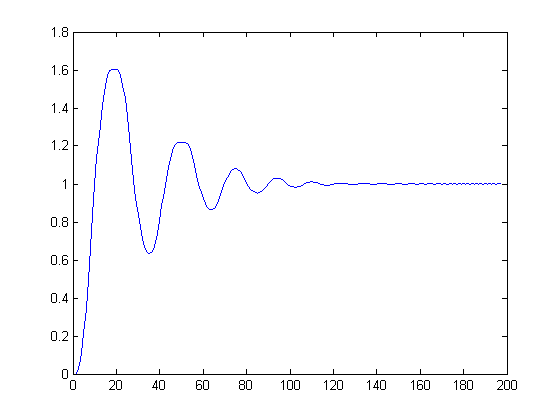
\includegraphics[width=0.6\textwidth]{modeloConst.png}
	\caption{modelo con entrada de voltaje constante}
	\label{fig:modeloConst}
\end{figure}

\begin{figure}[h!]
	\centering
	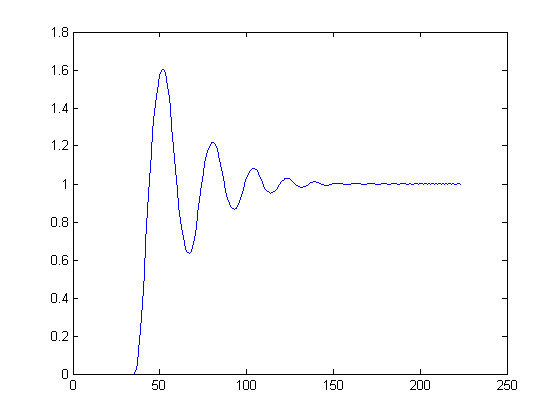
\includegraphics[width=0.6\textwidth]{modeloEscalon.png}
	\caption{modelo con entrada de voltaje señal Escalon}
	\label{fig:modeloEscalon}
\end{figure}

\begin{figure}[h!]
	\centering
	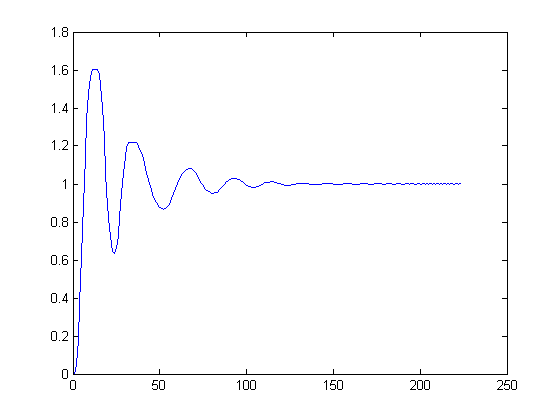
\includegraphics[width=0.6\textwidth]{modelo2Const.png}
	\caption{modelo con entrada de voltaje constante a partir de funcion de transferencia}
	\label{fig:modelo2Const}
\end{figure}

\begin{figure}[h!]
	\centering
	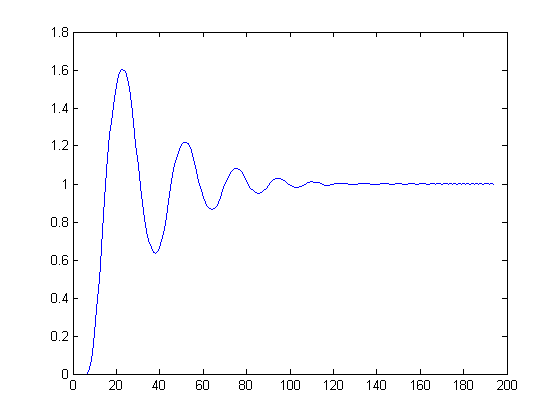
\includegraphics[width=0.6\textwidth]{modelo2Escalon.png}
	\caption{modelo con entrada de voltaje señal Escalon a partir de su función de transferencia}
	\label{fig:modelo2Escalon}
\end{figure}


\section{Análisis de Resultados}

\section{Conclusiones}

%\bibliographystyle{plain}
%\bibliography{Referencias.bib}
%\addbibresource{Referencias.bib}
\section{Referencias}

\begin{thebibliography}{widestlabel}
	\bibitem{MATLABWiki}\textsc{Wikipedia},\textsc{MATLAB},\textsc{https://en.wikipedia.org/wiki/MATLAB},\textit{},WikimediaGroup.
	
   \bibitem{Deepl}\textsc{Deepl},\textsc{www.DeepL.com/Translator}
	
	
	
\end{thebibliography}


\end{document}
